\documentclass[9pt,handout]{beamer}
\usepackage{etex} % Weird problem on dimentions
%\usetheme{spensiones}
%\mode<presentation> { \setbeamercovered{transparent} }
%\usepackage{stata}
\usepackage{tikz, tabularx, ulem}
%\usepackage{fancyvrb}
\usetikzlibrary{arrows, fit,positioning}

\title[{\tt parallel}]{Just tired of endless loops! \\ {\it \footnotesize or} {\normalsize {\tt parallel}: Stata module for parallel computing}}

\author[Vega, Quistorff]{George G. Vega\inst{1} \and Brian Quistorff\inst{2}}
\institute[USC and MSR]{\inst{1}University of Southern California\\ g.vegayon@gmail.com\and \inst{2}Microsoft AI and Resesarch\\Brian.Quistorff@microsoft.com}
\def\unix1{Intel Xeon X470 (hexadeca-core)}
\def\windows1{Intel i3 2120 (dual-core)}
\date{Stata Conference Baltimore\\July 27-28, 2017}
\begin{document}

\frame{
\maketitle
{\scriptsize
Thanks to Damian C. Clarke, F\'elix Villatoro and Eduardo Fajnzylber, Tom\'as Rau, 
Eric Melse, Valentina Moscoso, the 
Research team of the Chilean Pension Supervisor and several Stata users worldwide
for their valuable contributions.
The usual disclaimers applies.}
}

\frame{
\frametitle{Agenda}
\tableofcontents
}

\section{Motivation}

\begin{frame} % [allowframebreaks=.8]
\frametitle{Motivation}
\begin{itemize}
\item Despite the availability of administrative data, its exploitation is still a novel issue.\pause
\item At the same time, currently home computers are arriving with extremely high computational capabilities.\pause
\item Given its nature, matching both (big data problems and HPA) sounds strightforward.\pause
\item But, implementing parallel computing for the social scientiest is not easy,
\pause most of this due to lack of (user-friendly) statistical computing tools.\pause
\item {\tt parallel} aims to make a contribution to these issues.
\end{itemize}
\end{frame}

\section{What is and how does it work}

\frame{\tableofcontents[currentsection]}

\begin{frame} % [allowframebreaks=.8]
\frametitle{What is and how does it work}
\framesubtitle{What is?}

\begin{itemize}
\item Inspired in the R package ``snow''\pause (several other examples exists: StataMP, Condor HTC, C's Ox library, Matlab's Parallel Toolbox, etc.)\pause
\item Is designed to be used in multicore CPUs (dualcore, quadcore, etc.).\pause
\item It implements parallel computing methods through an OS's shell scripting (using Stata in batch mode) to accelerate computations.\pause
%\item By starting determined number of clusters (stata instances) this module was design to repeat a task simultaneously over the clusters.\pause
\item Depending on the task, can reach near to (or over) linear speedups proportional to the number of physical cores of the computer.\pause
\item Thus having a quad-core computer can lead to a 400\% speedup.
\end{itemize}

\end{frame}

\begin{frame}[b]
\frametitle{What is and how does it work}
\framesubtitle{How does it work?}
\begin{figure}
\centering
%\scalebox{.65}{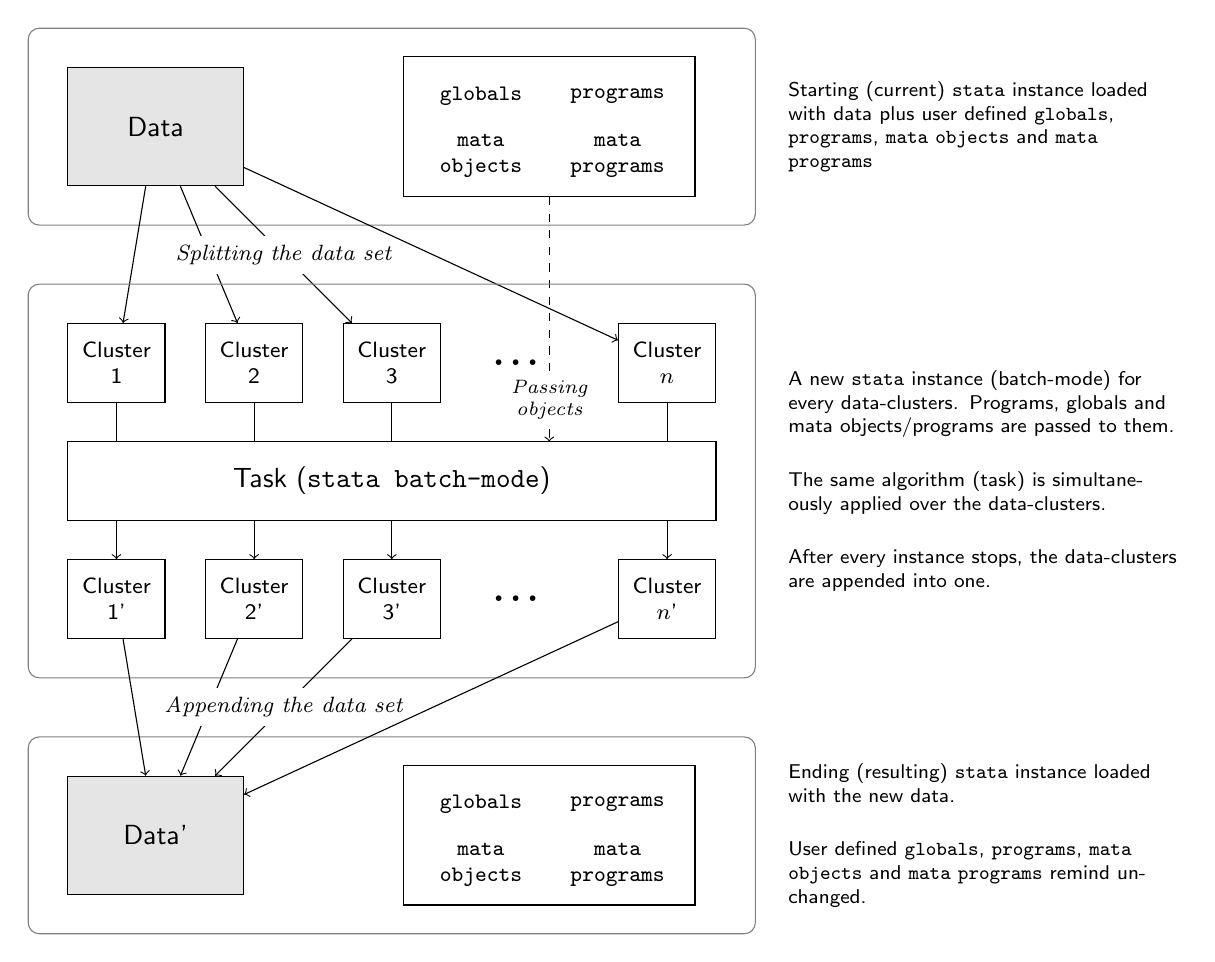
\begin{tikzpicture}[
	every node/.style={node distance=.5cm and .5cm, font=\sffamily}, 
	datablock/.style={rectangle, draw, fill=black!10, text width=2cm, minimum height=1.5cm, text badly centered},
	cluster/.style={rectangle, draw,text width=1cm, text badly centered, minimum height=1cm, font=\footnotesize\sffamily},
	explain/.style={rectangle, text width=5.5cm, align=left, font=\footnotesize\sffamily, node distance=.3, scale=.9}
	] 
	
\node [rectangle, draw=gray, text width=9cm, minimum height=2.5cm, rounded corners] (stata instance0) at (0,0) {};

% Original data
\node [datablock] (data) at (-3,0) {Data};
\matrix [
	draw=black,
	nodes={
		rectangle, text width=1.5cm, minimum height=.75cm, 
		scale=1,
		font=\tt\footnotesize, text badly centered}, column sep=0, row sep=0
	] (others) at (2,0) {
	\node {globals};& \node {programs}; \\
	\node {mata objects}; & \node {mata programs}; \\
};

% Data clusters
\node [cluster] (cluster3) at (0,-3) {Cluster 3};
\node [cluster, left=of cluster3] (cluster2) {Cluster 2};
\node [cluster, left=of cluster2] (cluster1) {Cluster 1};
\node [rectangle, right=of cluster3, text width=1cm, font=\Huge] (threepoints) {...};
\node [cluster, right=of threepoints,text badly centered] (clustern) {Cluster $n$};

% Splitting
\draw[->] (data) -- (cluster1);
\draw[->] (data) -- (cluster2);
\draw[->] (data) -- node [fill=white, font=\footnotesize\it] {Splitting the data set} (cluster3);
\draw[->] (data) -- (clustern);

\draw[->, dashed] (others) -- node [fill=white, font=\scriptsize\it, below=.65cm, text width=1.2cm, minimum height=.7cm,text badly centered] {Passing objects} (2,-4);

% Procesed clusters
\node [cluster] (cluster3p) at (0,-6) {Cluster 3'};
\node [cluster, left=of cluster3p] (cluster2p) {Cluster 2'};
\node [cluster, left=of cluster2p] (cluster1p) {Cluster 1'};
\node [rectangle, right=of cluster3p, text width=1cm, font=\Huge] (threepointsp) {...};
\node [cluster, right=of threepointsp,text badly centered] (clusternp) {Cluster $n$'};

\draw[->] (cluster1) -- (cluster1p);
\draw[->] (cluster2) -- (cluster2p);
\draw[->] (cluster3) -- (cluster3p);
\draw[->] (clustern) -- (clusternp);

% Task
\node [rectangle, draw=gray, text width=9cm, minimum height=5cm, rounded corners] (stata batch) at (0,-4.5) {};
\node [rectangle, fill=white, draw, text width=8cm, text badly centered,minimum height=1cm] (task) at (0,-4.5) {Task (\texttt{stata batch-mode})};

% Result
\node [rectangle, draw=gray, text width=9cm, minimum height=2.5cm, rounded corners] (stata instance1) at (0,-9) {};
\node [datablock] (datap) at (-3,-9) {Data'};
\matrix [
	draw=black,
	nodes={
		rectangle, text width=1.5cm, minimum height=.75cm, 
		scale=1,
		font=\tt\footnotesize, text badly centered}, column sep=0, row sep=0
	] (othersp) at (2,-9) {
	\node {globals};& \node {programs}; \\
	\node {mata objects}; & \node {mata programs}; \\
};

\draw[->] (cluster1p) -- (datap);
\draw[->] (cluster2p) -- (datap);
\draw[->] (cluster3p) -- node [fill=white, font=\footnotesize\it] {Appending the data set} (datap);
\draw[->] (clusternp) -- (datap);

% Text
\node [explain, right=of stata instance0] {Starting (current) {\tt stata} instance loaded with data plus user defined {\tt globals}, {\tt programs}, {\tt mata objects} and {\tt mata programs}};

\node [explain, right=of stata batch] {A new {\tt stata} instance (batch-mode) for every data-clusters. Programs, globals and mata objects/programs are passed to them.\\\bigskip The same algorithm (task) is simultaneously applied over the data-clusters.\\\bigskip After every instance stops, the data-clusters are appended into one.};

\node [explain, right=of stata instance1] {Ending (resulting) {\tt stata} instance loaded with the new data.\\\bigskip User defined {\tt globals}, {\tt programs}, {\tt mata objects} and {\tt mata programs} remind unchanged.};

\end{tikzpicture}}
\scalebox{.7}{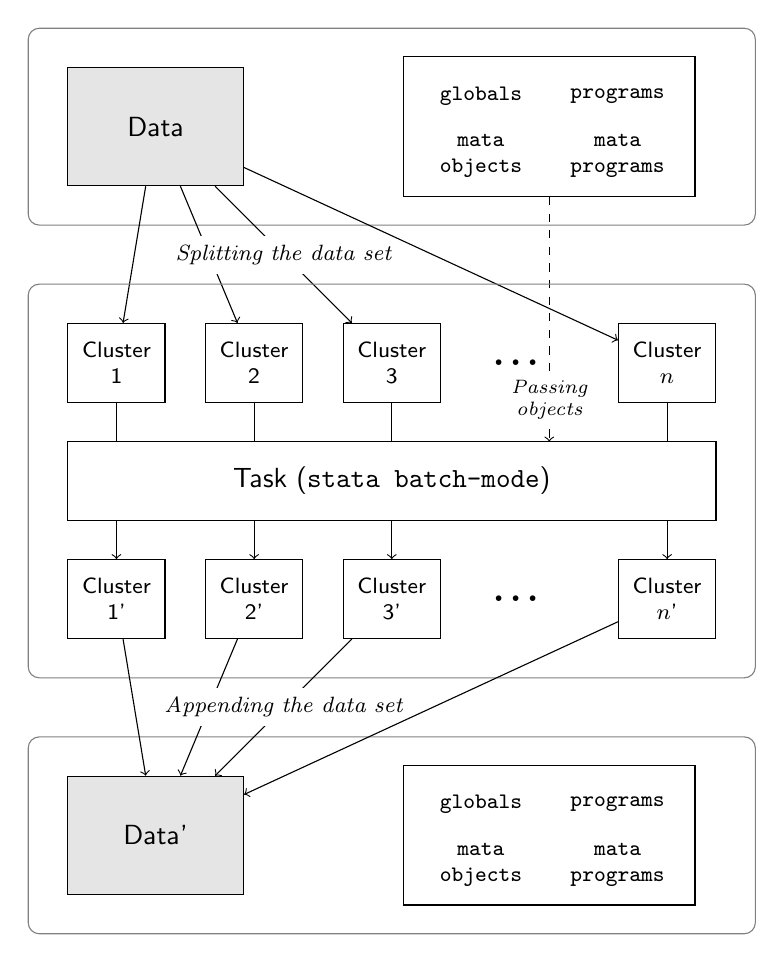
\begin{tikzpicture}[
	every node/.style={node distance=.5cm and .5cm, font=\sffamily}, 
	datablock/.style={rectangle, draw, fill=black!10, text width=2cm, minimum height=1.5cm, text badly centered},
	cluster/.style={rectangle, draw,text width=1cm, text badly centered, minimum height=1cm, font=\footnotesize\sffamily},
	explain/.style={rectangle, text width=5.5cm, align=left, font=\footnotesize\sffamily, node distance=.3, scale=.9}
	] 
	
\node [rectangle, draw=gray, text width=9cm, minimum height=2.5cm, rounded corners] (stata instance0) at (0,0) {};

% Original data
\node [datablock] (data) at (-3,0) {Data};
\matrix [
	draw=black,
	nodes={
		rectangle, text width=1.5cm, minimum height=.75cm, 
		scale=1,
		font=\tt\footnotesize, text badly centered}, column sep=0, row sep=0
	] (others) at (2,0) {
	\node {globals};& \node {programs}; \\
	\node {mata objects}; & \node {mata programs}; \\
};

% Data clusters
\node [cluster] (cluster3) at (0,-3) {Cluster 3};
\node [cluster, left=of cluster3] (cluster2) {Cluster 2};
\node [cluster, left=of cluster2] (cluster1) {Cluster 1};
\node [rectangle, right=of cluster3, text width=1cm, font=\Huge] (threepoints) {...};
\node [cluster, right=of threepoints,text badly centered] (clustern) {Cluster $n$};

% Splitting
\draw[->] (data) -- (cluster1);
\draw[->] (data) -- (cluster2);
\draw[->] (data) -- node [fill=white, font=\footnotesize\it] {Splitting the data set} (cluster3);
\draw[->] (data) -- (clustern);

\draw[->, dashed] (others) -- node [fill=white, font=\scriptsize\it, below=.65cm, text width=1.2cm, minimum height=.7cm,text badly centered] {Passing objects} (2,-4);

% Procesed clusters
\node [cluster] (cluster3p) at (0,-6) {Cluster 3'};
\node [cluster, left=of cluster3p] (cluster2p) {Cluster 2'};
\node [cluster, left=of cluster2p] (cluster1p) {Cluster 1'};
\node [rectangle, right=of cluster3p, text width=1cm, font=\Huge] (threepointsp) {...};
\node [cluster, right=of threepointsp,text badly centered] (clusternp) {Cluster $n$'};

\draw[->] (cluster1) -- (cluster1p);
\draw[->] (cluster2) -- (cluster2p);
\draw[->] (cluster3) -- (cluster3p);
\draw[->] (clustern) -- (clusternp);

% Task
\node [rectangle, draw=gray, text width=9cm, minimum height=5cm, rounded corners] (stata batch) at (0,-4.5) {};
\node [rectangle, fill=white, draw, text width=8cm, text badly centered,minimum height=1cm] (task) at (0,-4.5) {Task (\texttt{stata batch-mode})};

% Result
\node [rectangle, draw=gray, text width=9cm, minimum height=2.5cm, rounded corners] (stata instance1) at (0,-9) {};
\node [datablock] (datap) at (-3,-9) {Data'};
\matrix [
	draw=black,
	nodes={
		rectangle, text width=1.5cm, minimum height=.75cm, 
		scale=1,
		font=\tt\footnotesize, text badly centered}, column sep=0, row sep=0
	] (othersp) at (2,-9) {
	\node {globals};& \node {programs}; \\
	\node {mata objects}; & \node {mata programs}; \\
};

\draw[->] (cluster1p) -- (datap);
\draw[->] (cluster2p) -- (datap);
\draw[->] (cluster3p) -- node [fill=white, font=\footnotesize\it] {Appending the data set} (datap);
\draw[->] (clusternp) -- (datap);

% Text
%\node [explain, right=of stata instance0] {Starting (current) {\tt stata} instance loaded with data plus user defined {\tt globals}, {\tt programs}, {\tt mata objects} and {\tt mata programs}};

%\node [explain, right=of stata batch] {A new {\tt stata} instance (batch-mode) for every data-clusters. Programs, globals and mata objects/programs are passed to them.\\\bigskip The same algorithm (task) is simultaneously applied over the data-clusters.\\\bigskip After every instance stops, the data-clusters are appended into one.};

%\node [explain, right=of stata instance1] {Ending (resulting) {\tt stata} instance loaded with the new data.\\\bigskip User defined {\tt globals}, {\tt programs}, {\tt mata objects} and {\tt mata programs} remind unchanged.};

\end{tikzpicture}
}
\end{figure}
\end{frame}

\begin{frame}
\frametitle{What is and how does it work}
{\Large Sounds ``pretty'' but...}\pause {\Huge is this for real!?}
\end{frame}

\begin{frame}
\frametitle{What is and how does it work}
\framesubtitle{Parallel's backend}

When the user enters 

\begin{figure}[fragile]
\small
\centering
{\bf{\tt parallel: gen n = \_N}}
\end{figure} 

{\tt parallel} takes the command and writes something like this\pause
\bigskip
\scriptsize

%\scalebox{.9}{
\def\anchomini{.6\textwidth}
\begin{minipage}[c]{\anchomini}
\begin{semiverbatim}
  cap clear all
  cd ~
1 {\bf{}set seed 34815}
  set memory 16777216b
  cap set maxvar 5000
  cap set matsize 400
2 {\bf{}local pll\_instance 1}
  local pll_id efcql2tspr
  capture \{
  noisily \{
3 {\bf{}use \_\_pllefcql2tsprdataset if \_efcql2tsprcut == 1}
  {\bf{}gen n = \_N}
  \}
  \}
4 {\bf{}save \_\_pllefcql2tsprdta1, replace}
  local result = _rc
  cd ~
5 {\bf{}mata: write\_diagnosis(st\_local("result"),}
  >{\bf{}"\_\_pllefcql2tsprfinito1")}
\end{semiverbatim}
\end{minipage}\pause{}
% SPLIT
\begin{minipage}[c]{\anchomini}
\begin{semiverbatim}
  cap clear all
  cd ~
1 {\bf{}set seed 98327}
  set memory 16777216b
  cap set maxvar 5000
  cap set matsize 400
2 {\bf{}local pll\_instance 2}
  local pll_id efcql2tspr
  capture \{
  noisily \{
3 {\bf{}use \_\_pllefcql2tsprdataset if \_efcql2tsprcut == 2}
  {\bf{}gen n = \_N}
  \}
  \}
4 {\bf{}save \_\_pllefcql2tsprdta2, replace}
  local result = _rc
  cd ~
5 {\bf{}mata: write\_diagnosis(st\_local("result"),}
  >{\bf{}"\_\_pllefcql2tsprfinito2")}
\end{semiverbatim}
\end{minipage}

%}
\end{frame}

\begin{frame}
\frametitle{What is and how does it work}
{\Large Ok, it works but...}\pause 

{\Huge it must be really hard to use!}
\end{frame}

\section{Benchmarks}
\frame{\tableofcontents[currentsection]}

\begin{frame}[b,fragile]
\frametitle{Benchmarks}
\framesubtitle{Simple example: Serial replace}

\begin{minipage}[c]{1\textwidth}
\begin{minipage}[c]{.35\textwidth}
Serial fashion
\begin{semiverbatim}\scriptsize
do mydofile.do
\end{semiverbatim}
Parallel fashion
\begin{semiverbatim}\scriptsize
parallel do mydofile.do
\end{semiverbatim}
\end{minipage}
%SPLIT
\fbox{
\begin{minipage}[c]{.6\textwidth}\scriptsize
\begin{figure}
\caption{mydofile.do}
\begin{semiverbatim}
local size = \_N

forval i=1/`size' \{

\hspace{1cm}qui replace x = ///

\hspace{1.5cm}1/sqrt(2*`c(pi)')*exp(-(x\^{}2/2)) in `i'

\}
\end{semiverbatim}
\end{figure}
\end{minipage}}
\end{minipage}

\begin{table}[!h]
\centering
\caption{Serial replacing using a loop on a Linux Server (16 clusters)}
\scalebox{.9}{
\begin{tabular}{l*{3}{c}}\hline
& 100.000 &         1.000.000 &       10.000.000 \\ \hline
CPU &     1.43 &     16.94 &    144.68 \\
Total &     0.34 &      3.20 &     12.49 \\
\hspace{2mm} Setup &     0.00 &      0.00 &      0.00 \\
\hspace{2mm} Compute &     0.32 &      3.07 &     11.54 \\
\hspace{2mm} Finish &     0.02 &      0.12 &      0.95 \\
\hline Ratio (compute) &     4.50 &      5.51 &     12.53 \\
Ratio (total) &     4.22 (26\%) &      5.30 (30\%) &     11.58 (72\%) \\
\hline
\multicolumn{4}{l}{\footnotesize Tested on a \unix1 machine}
\end{tabular}}
\end{table}

\end{frame}

\begin{frame}[b,fragile]
\frametitle{Benchmarks}
\framesubtitle{Monte Carlo simulation (Windows Machine)}
\begin{minipage}[c]{1\textwidth}
\begin{minipage}[c]{.45\textwidth}
\bigskip
Serial fashion
\begin{semiverbatim}\scriptsize
do myexperiment.do
\end{semiverbatim}
Parallel fashion
\begin{semiverbatim}\scriptsize
parallel do myexperiment.do, nodata
\end{semiverbatim}
\end{minipage}
%SPLIT
\fbox{
\scalebox{.4}{
\begin{minipage}[c]{1\textwidth}\scriptsize
\begin{figure}
{\Huge \caption{myexperiment.do}}
\begin{semiverbatim}
local num\_of\_intervals = 50

if length("`pll\_id'") == 0 \{

\hspace{.5cm}local start = 1

\hspace{.5cm}local end = `num\_of\_intervals'

\}

else \{

\hspace{.5cm}local ntot = floor(`num\_of\_intervals'/\$PLL\_CLUSTERS)

\hspace{.5cm}local start = (`pll\_instance' - 1)*`ntot' + 1

\hspace{.5cm}local end = (`pll\_instance')*`ntot'

\hspace{.5cm}if `pll\_instance' == \$PLL\_CLUSTERS local end = 10

\}

local reps 10000

forval i=`start'/`end' \{

\hspace{.5cm}qui use census2, clear

\hspace{.5cm}gen true\_y = age

\hspace{.5cm}gen z\_factor = region

\hspace{.5cm}sum z\_factor, meanonly

\hspace{.5cm}scalar zmu = r(mean)

\hspace{.5cm}qui \{

\hspace{.5cm}\hspace{.5cm}gen y1 = .

\hspace{.5cm}\hspace{.5cm}gen y2 = .

\hspace{.5cm}\hspace{.5cm}local c = `i'

\hspace{.5cm}\hspace{.5cm}set seed `c'

\hspace{.5cm}\hspace{.5cm}simulate c=r(c) mu1=r(mu1) se\_mu1 = r(se\_mu1) ///

\hspace{.5cm}\hspace{.5cm}\hspace{.5cm}\hspace{.5cm}mu2=r(mu2) se\_mu2 = r(se\_mu2), /// 

\hspace{.5cm}\hspace{.5cm}\hspace{.5cm}\hspace{.5cm}saving(cc`i', replace) nodots reps(`reps'): ///

\hspace{.5cm}\hspace{.5cm}\hspace{.5cm}\hspace{.5cm}mcsimul1, c(`c')

\hspace{.5cm}\}

\}
\end{semiverbatim}
\end{figure}
\end{minipage}}}
\end{minipage}
\begin{table}[!h]
\centering
\caption{Monte Carlo Experiment on a Windows Machine (4 clusters)}
\scalebox{.85}{
\begin{tabular}{l*{2}{c}}\hline
& 2 &               4 \\ \hline
CPU &   111.49 &    114.13 \\
Total &    58.02 &     37.48 \\
\hspace{2mm} Setup &     0.00 &      0.00 \\
\hspace{2mm} Compute &    58.02 &     37.48 \\
\hspace{2mm} Finish &     0.00 &      0.00 \\
\hline Ratio (compute) &     1.92 &      3.04 \\
Ratio (total) &     1.92 (96\%)&      3.04 (76\%)\\
\hline
\multicolumn{3}{l}{\footnotesize Tested on a \windows1 machine}
\end{tabular}}
\end{table}
\end{frame}

\begin{frame}[b]
\frametitle{Benchmarks}
\framesubtitle{Monte Carlo simulation (Unix Machine)}
\bigskip
Serial fashion
\begin{semiverbatim}
\scriptsize
do myexperiment.do
\end{semiverbatim}

Parallel fashion
\begin{semiverbatim}
\scriptsize
parallel do myexperiment.do, nodata
\end{semiverbatim}

\begin{table}[!h]
\centering
\caption{Monte Carlo Experiment on a Linux Server (16 clusters)}
\scalebox{.85}{
\begin{tabular}{l*{4}{c}}\hline
& 2 &               4 &               8 &              16 \\ \hline
CPU &   164.79 &    164.04 &    162.84 &    163.89 \\
Total &    69.85 &     34.28 &     19.00 &     10.78 \\
\hspace{2mm} Setup &     0.00 &      0.00 &      0.00 &      0.00 \\
\hspace{2mm} Compute &    69.85 &     34.28 &     19.00 &     10.78 \\
\hspace{2mm} Finish &     0.00 &      0.00 &      0.00 &      0.00 \\
\hline Ratio (compute) &     2.36 &      4.78 &      8.57 &     15.21 \\
Ratio (total) &     2.36 (118\%) &      4.78 (120\%)&      8.57 (107\%) &     15.21 (95\%) \\
\hline
\multicolumn{4}{l}{\footnotesize Tested on a \unix1 machine}
\end{tabular}}
\end{table}

\end{frame}

\begin{frame}[b]
\frametitle{Benchmarks}
\framesubtitle{Reshaping Administrative Data}
\bigskip
Serial fashion
\begin{semiverbatim}
\scriptsize
reshape wide tipsolic rutemp opta derecho ngiros, ///

\hspace{1cm}i(id) j(time)
\end{semiverbatim}

Parallel fashion
\begin{semiverbatim}
\scriptsize
parallel, by(id) :reshape wide tipsolic rutemp opta derecho ngiros, ///

\hspace{1cm}i(id) j(time)
\end{semiverbatim}

\begin{table}[!h]
\centering
\caption{Reshaping wide a large database on a Linux Server (8 clusters)}
\scalebox{.8}{
\begin{tabular}{l*{3}{c}}\hline
& 100.000 &         1.000.000 &         5.000.000 \\ \hline
CPU &     5.51 &     72.70 &    392.97 \\
Total &     2.33 &     17.46 &     86.44 \\
\hspace{2mm} Setup &     0.00 &      0.00 &      0.00 \\
\hspace{2mm} Compute &     1.83 &     12.42 &     57.93 \\
\hspace{2mm} Finish &     0.50 &      5.04 &     28.51 \\
\hline Ratio (compute) &     3.01 &      5.85 &      6.78 \\
Ratio (total) &     2.37 (29\%)&      4.16 (52\%)&      4.55 (57\%)\\
\hline
\multicolumn{4}{l}{\footnotesize Tested on a \unix1 machine}
\end{tabular}}
\end{table}

\end{frame}

\section{Syntax and Usage}

\frame{\tableofcontents[currentsection]}

\begin{frame}
\frametitle{Syntax and Usage}

Setup

\begin{semiverbatim}
\footnotesize
{\bf parallel setclusters} {\it \#}  [, \uline{f}orce] 
\end{semiverbatim}\pause

By syntax

\begin{semiverbatim}
\footnotesize
{\bf parallel} [, by({\it \color{blue} varlist}) \uline{p}rograms \uline{m}ata \uline{s}eeds({\it \color{blue} string}) \uline{r}andtype({\it \color{blue} random.org$|$datetime})

\hspace{1cm} \uline{pr}ocessors({\it \color{blue} integer}) \uline{nod}ata]:  {\it stata\_cmd}
\end{semiverbatim}\pause

Do syntax

\begin{semiverbatim}
\footnotesize
{\bf parallel do} {\it \color{blue} filename}

\hspace{1cm} [, by({\it \color{blue} varlist}) \uline{p}rograms \uline{m}ata \uline{s}eeds({\it \color{blue} string}) \uline{r}andtype({\it \color{blue} random.org$|$datetime})

\hspace{1cm} \uline{pr}ocessors({\it \color{blue} integer}) \uline{nod}ata]
\end{semiverbatim}

\end{frame}


\begin{frame}
\frametitle{Syntax and Usage}
\framesubtitle{Recomendations on its usage}

\begin{columns}
\begin{column}{.5\textwidth}
{\color{gray}
{\tt parallel suit ...}
\rule{\linewidth}{4pt}}
\begin{itemize}
\item Montecarlo simulation.\pause
\item Extensive nested control flow (loops, while, ifs, etc.).\pause
\item Bootstraping/Jacknife.\pause
\item Simulations in general.\pause
\end{itemize}
\end{column}%
\hfill%
\begin{column}{.5\textwidth}
{\color{gray}
{\tt parallel doesn't suit ...}
\rule{\linewidth}{4pt}}
\begin{itemize}
\item (already) fast commands.\pause
\item Regressions, ARIMA, etc.\pause
\item Linear Algebra.\pause
\item Whatever StataMP does better.
\end{itemize}
\end{column}%
\end{columns}
\end{frame}

\section{Concluding Remarks}

\begin{frame}
\frametitle{Concluding Remarks}

\begin{itemize}
\item In the case of Stata, {\tt parallel} is, to the authors knowledge, the first public user-contribution to parallel computing\pause
\item its major strengths/advantages are in simulation models and non-vectorized operations such as control-flow statements.\pause
\item Depending on the proportion of the algorithm that can be de-serialized, it is possible to reach near to constant scale speedups.\pause
\item {\tt parallel} establishes a new basis for parallel computing in Stata,\pause{}
thus an all new set of algorithms can be implemented:\pause
\begin{itemize}
\item {\tt parsimulate}\pause
\item {\tt parfor}\pause
\item {\tt parbootstrap}\pause
\item {\tt parnnmatch}\pause
\item ... {\large You name it!}
\end{itemize}
\end{itemize}

\end{frame}

\title{Thank you very much!}

\frame{\maketitle
}

\end{document}
